\section{I/O}

处理器必须像和主存交互一样同设备交互。x86 处理提供了特殊的 in, out 指令来在设备地址(称为'I/O 端口') 上读写。这两个指令的硬件实现本质上和读写内存是相同的。早期的 x86 处理器有一条附加的地址线:0表示从 I/O 端口读写,1则表示从主存读写。每个硬件设备会处理它所在 I/O 端口所接收到的读写操作。设备的端口使得软件可以配置设备,检查状态,使用设备;例如,软件可以通过对 I/O 端口的读写,使磁盘接口硬件对磁盘扇区进行读写。

很多计算机体系结构都没有单独的设备访问指令,取而代之的是让设备拥有固定的内存地址,然后通过内存读写实现设备读写。实际上现代 x86 体系结构就在大多数高速设备上(如网络、磁盘、显卡控制器)使用了该技术,叫做 内存映射 I/O。但由于向前兼容的原因, in, out 指令仍能使用,而比较老的设备如 xv6 中使用的 IDE 磁盘控制器仍使用这两个指令。

Xv6系统的I/O主要面向3个设备:磁盘,键盘,屏幕。

磁盘I/O控制方式为程序直接控制(查询)方式。调用磁盘ide驱动来进行硬件读写,向上提供统一的open,read,write等接口。

键盘输入方式为中断控制方式。将键盘中断捕获,交给控制台输入。

屏幕显示方式为程序直接控制(查询)方式。调用显示驱动向cga接口输出字符信息。

首先,我们从用户模式介绍xv6.

\subsection{I/O 系统调用部分}

\subsection{使用系统调用的文件描述符}

\begin{minted}{C}
read (int fd, char* buf, int len);
write (int fd, char* buf, int len);
stat (int fd, struct stat * );
dup (int fd);
close (int fd);
\end{minted}

\subsubsection{命名服务}

\begin{minted}{C}
link (char ∗ oldpath , char ∗ newpath);
fd = open (char ∗ path , int flags);
unlink (char ∗ path);
mkdir (char ∗ path );
rmdir (char ∗ path );
\end{minted}

还有管道函数用作文件缓冲

\begin{minted}{C}
pipe (int pipefd[2]);
\end{minted}

然后,我们开始进入xv6的核心

xv6核心是一个分层系统,其中文件层由pipe子系统和inode子系统组成,inode子系统包括name层、inode层、buffer层和driver层, 系统调用调用文件层,name层和inode层。

简单的介绍后,我们来探讨一下xv6如何在不同的硬件,结构和函数方法下,向用户模式提供统一的界面。

xv6 文件的抽象格式如下:

\begin{minted}{C}
struct file{
enum {FD_NONE, FD_PIPE , FD_INODE} type;
int ref; // reference count
char readable;
char writeable;
struct pipe∗ pipe;
struct inode ∗ ip;
uint off;
};
\end{minted}

其中各个变量功能下文均有解释,并且均将细化到代码模块

\subsection{I/O 子系统}

子系统由以下几个模块组成:

\begin{itemize}
\item FD\_PIPE.
\item FD\_INODE:
\item T\_FILE, T\_DIR, T\_DEV.
\end{itemize}

每个 I/O 子系统都是由一个结构体和一个操作集合来定义的,子系统中的各个模块将在下文予以解释

  FD\_PIPE模块

  \begin{minted}{C}
struct pipe{
struct spinlock lock;
char data[PIPESIZE];
uint nread;//读取的字符数目
uint nwrite;//写入的字符数目
intreadopen;//读取的文件仍然开启
intwriteopen;/写入的文件仍然开启
};
  \end{itemize}

  还有pipe的一些相关基本操作

  pipalloc, pipeclose, piperead, pipewrite.

  FD\_INODE模块

\begin{minted}{C}
struct inode{
uint dev;//设备数字
uint inum;//Inode数字
int ref;//Reference count
int flags;//IBUSY,IVALID
short type;// inode的磁盘镜像
short major;
short minor;
short nlink;
uint size;
uint addrs[NDIRECT+1];
};
\end{minted}

F\_INODE相关方法
Listing1:读入T\_FILE or T\_DIR
调用如下方法
namei, create, ilock, readi, writei, stati, iunlock, iput
Listing2:读入T\_DEV
consoleread, consolewrite

文件层的系统调用

sys dup, sys read, sys write, sys fstat, sys close.

在fd系统调用中使用的函数

\begin{minted}{C}
struct file ∗ filedup(struct file ∗f)
fileclose(struct file ∗f);
fileread(struct file ∗f, char ∗buf, int len);
filewrite(struct file ∗f,char∗ buf, int len);
filestat(struct file∗f, struct stat∗s);
\end{minted}

fdalloc:用于返回最低限度的被数字标记的空余文件槽.

\begin{minted}{C}
static int fdalloc(struct file ∗f){
int fd;
for(fd = 0;fd < NOFILE; fd ++){
if(proc−>ofile[fd]==0){
proc−>ofile[fd] = f;
return fd;
}
}
return −1;
}
\end{minted}

sys\_dup部分

\begin{minted}{C}
sys_dup(void){
struct file ∗f;
int fd;
if(argfd(0,0,&f)<0) return −1;
if((fd = fdalloc(f))<0) return −1;
filedup(f);
return fd;
}
\end{minted}

sys\_read部分

\begin{minted}{C}
int sys_read(void){
struct file ∗f;
int n;
char ∗p;
if(argfd(0,0,&f)<0||argint(2,&n)<0||argptr(1,&p,n)<0) return −1;
return fileread(f,p,n);
}
\end{minted}
sys\_write部分
\begin{minted}{C}
int sys_write(void){
struct file ∗f;
int n;
char ∗p;
if(argfd(0,0,&f)<0||argint(2,&n)<0||argptr(1,&p,n)<0) return −1;
return filewrite(f,p,n);
}
\end{minted}
sys\_fstat部分
\begin{minted}{C}
int sys_fstat(void){
struct file ∗f;
struct stat ∗st;
if(argfd(0,0,&f)<0||argptr(1,(void∗)&st,sizeof(∗st))<0) return−1;
return filestat(f,st);
}
\end{minted}
sys\_close部分
\begin{minted}{C}
int sys_close(void){
int fd;
struct file∗f;
if(argfd(0,&fd,&f)<0) return −1;
proc−>ofile[fd]=0;
fileclose(f);
return 0;
}
\end{minted}

文件层的实现通过以下五个函数:

filedup,fileread,filewrite,filestat,fileclose.

我们先来看一下ofile/file/inode/pipe 的执行流程

1. 无文件开启时

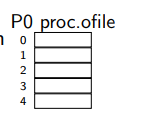
\includegraphics[width=6in]{figures/eg_file/image156.png}

2. 执行open(”/carmi/f0”)

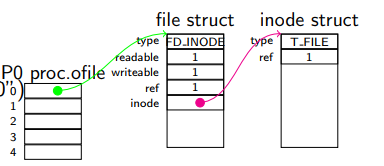
\includegraphics[width=6in]{figures/eg_file/image157.png}

3. 执行dup(0)

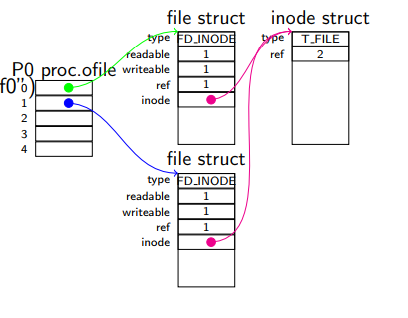
\includegraphics[width=6in]{figures/eg_file/image158.png}

4. 执行close(0)

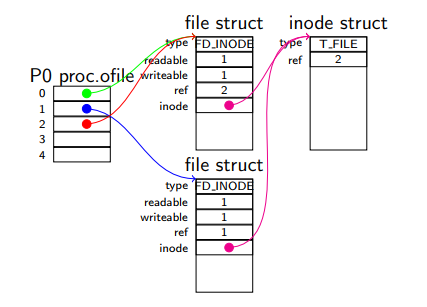
\includegraphics[width=6in]{figures/eg_file/image159.png}

5. 执行dup(1)

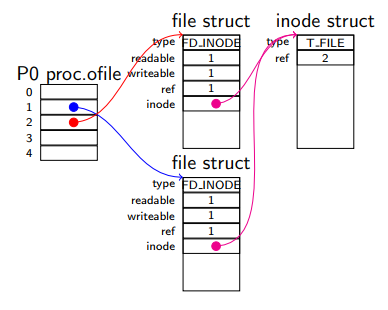
\includegraphics[width=6in]{figures/eg_file/image160.png}

6. 执行open(”/console”)

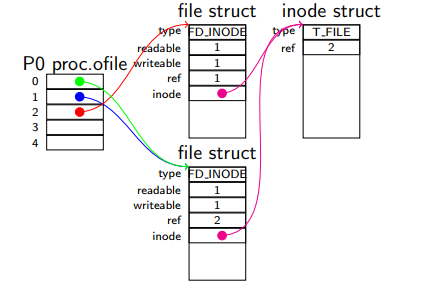
\includegraphics[width=6in]{figures/eg_file/image161.png}

7. 执行fork()

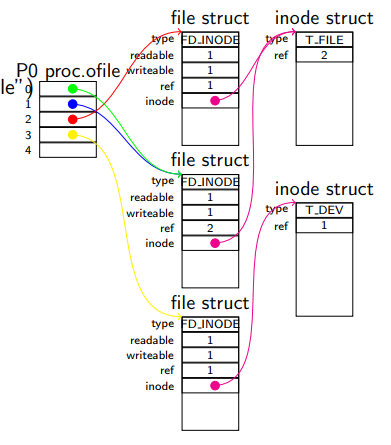
\includegraphics[width=6in]{figures/eg_file/image162.png}

8. 执行P0 close(1)

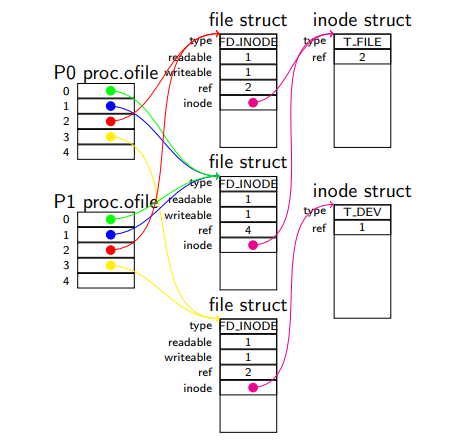
\includegraphics[width=6in]{figures/eg_file/image163.png}

9. 执行P1 close(2)

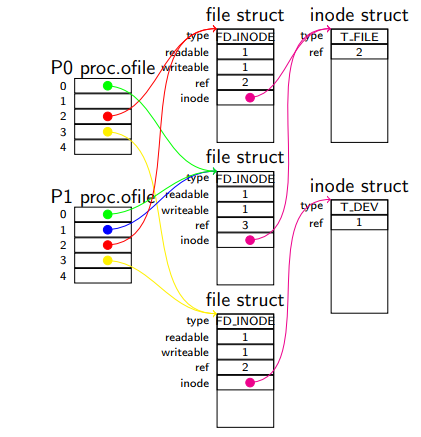
\includegraphics[width=6in]{figures/eg_file/image164.png}

10. 执行P0 pipe()

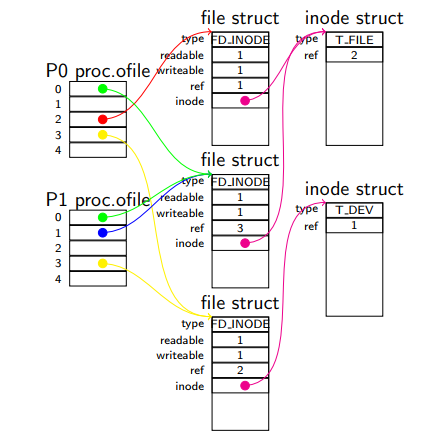
\includegraphics[width=6in]{figures/eg_file/image165.png}



文件层调度

文件层将调度一下子系统之一:

1.pipe.
2.inode.
pipe子系统和inode层使用的函数
Pipe子系统:
\begin{itemize}
\item piperead(pipe *p, char *addr, int len);
\item pipewrite(pipe *p ,char *addr, int len);
\item pipeclose(pipe *p ,int writeside);
\end{itemize}

inode子系统:
\begin{itemize}
\item ilock(inode *ip);
\item iunlock(inode *ip);
\item readi(inode *ip, char *adr, int len);
\item writei(inode *ip, char* adr, int len);
\item iput(inode *ip);
\item •stati(inode *ip, stat* stat);
\item begintrans();
\item committrans();
\end{itemize}


模块详细说明

file\_dup模块

\begin{minted}{C}
struct file∗ file_dup(struct file∗f){
acquire(&ftable.lock);
if(f−>ref<1) panic(”filedup”);
f−>ref++;
release(&ftable.lock);
return f;
}
\end{minted}

根据类型,file\_read将读取委托给以下其中一个:

管道,readi。

对于FD\_INODE类型,处理文件位置。

file\_read模块

\begin{minted}{C}
int file_read(structfile ∗f, char ∗addr,int n){
int r;
if(f−>readable==0) return −1;
if(f−>type==FDPIPE) return pipe_read(f−>pipe,addr,n);
if(f−>type==FDINODE){
ilock(f−>ip);
if((r=readi(f−>ip,addr,f−>off,n))>0) f−>off+=r;
iunlock(f−>ip);
return r;
}
panic(”fileread”);
}
\end{minted}

根据类型,filewrite将写入委托给以下其中一个:

pipe写入,writei。

对于FD\_INODE类型,处理文件位置。

file\_write模块


\begin{minted}{C}
int file_write(struct file ∗f, char∗ addr, int n){
if(f−>writable==0) return−1;
if(f−>type==FDPIPE) return pipe_write(f−>pipe,addr,n);
if(f−>type==FDINODE){
int max=((LOGSIZE−1−1−2)/2)∗512;
for(int i=0;i<n;){
int n1=n−i;
if(n1>max) n1=max;
begintrans();
ilock(f−>ip);
if((r=writei(f−>ip,addr+i,f−>off,n1))>0) f−>off+=r;
iunlock(f−>ip);
committrans();
if(r<0) break;
if(r!=n1) panic(”shortfilewrite”);
i+=r;
}
return i==n ? n:−1;
}
panic(”filewrite”);
}
\end{minted}

reference count已更新。

如果reference count下降到零,我们委托给其中一个:

pipe关闭, iput。

由于iput我们必须释放需要注意,因此需要

复制文件结构。

file\_stat模块

\begin{minted}{C}
int file_stat(structfile ∗f,structstat ∗st){
if(f−>type==FDINODE){
ilock(f−>ip);
stati(f−>ip,st);
iunlock(f−>ip);
return 0;
}
return −1;
}
\end{minted}

file\_close模块

\begin{minted}{C}
void file_close(struct file ∗f){
  acquire(&ftable.lock);
  if(f−>ref<1) panic(”fileclose”);
  if(−−f−>ref>0){
    release(&ftable.lock);
    return;
  }
  structff=∗f;
  f−>ref=0;
  f−>type=FDNONE;
  release(&ftable.lock);
  if(ff.type==FDPIPE) pipeclose(ff.pipe,ff.writable);
  else if(ff.type==FDINODE){
    begintrans();iput(ff.ip);committrans();
  }
}
\end{minted}

\subsection{I/O缓存Buf结构}

xv6用buf对磁盘上的block块进行缓存。buf是一个LRU链表。也就说最近访问的buf总是放在链表的首部。

bio.c

binit是将整个buf链表初始化,并将其链成一个表。bget则寻找一个扇区的buf。首先在buf链表中寻找是否有此扇区的buf,如果没有的话,则加入开辟一个新的buf存储扇区。bread是读取某一个扇区。首先通过bget找到相应的buf。如果发现状态不是B\_VALID,则通过ide\_rw进行磁盘同步。bwrite是将buf中的内容写入扇区。调用bwrite之前需要在外部对buf,从而保证一致性。brelse是用来释放buf。这个函数是当对buf访问结束时调用的。此时基于LRU算法,将把buf放在buf链表的头部。

ide.c

此文件是对ide磁盘进行读写操作。I/O读写是异步的。

其中主要的流程如下:首先看ide\_rw。对于每个读写操作,都有一个ide\_queue进行排队。在ide\_rw函数中,会把当前的进程加入到ide\_queue中。如果之前disk没有开始读写,则唤起disk读写。(141~142行)。然后在145~146进行轮询等待读写进程的完成。轮询中并不是盲等,而是会sleep当前进程,等待进程完成是被唤起。

  ide\_start\_request过程是将buf b进程请求发送到磁盘。当进程完成时,磁盘将发出完成的硬件中断。ide\_intr则是相应此中断的过程。ide\_intr将在106~108行清除状态,并唤醒等待此buf的进程。最后如果此进程在ide\_queue有后继进程,则启动此进程。

  APIC

  在对称多处理实现中,CPU需要处理各个设备发来的中断,我们将这种中断纳入I/O的管理。

  APIC(Advanced Programmable Interrupt Controller)是一个与8259A兼容的高级中断处理器。它不但实现了中断处理的功能,还实现了以下功能:

  1. 提供与中断相关的设备通讯

2. 提供多处理器(或多CPU)之间的中断共享与中断通讯

事实上,xv6与外部设备的很大一部分通讯处理,都是通过APIC来实现的。

APIC分为两层:Local APIC和I/O APIC。

a. I/O APIC

I/O APIC是用来与外部设备通讯的,它完成了APIC最主要的功能:中断处理。

I/O APIC提供了两个模式,普通模式和8259A兼容模式。xv6在单核环境下,会选择使用8259A兼容模式,而在多处理器环境下,则会使用普通模式。

b. Local APIC

Local APIC是APIC的顶层,每个核都有一个对应的Local APIC。它负责进行多处理器之间的中断传输,屏蔽中断,还提供了一个可编程的Timer。由于I/O APIC已经提供了中断处理的功能,Local APIC只是起辅助作用,可以屏蔽不用。

xv6在单核环境中,Local APIC被屏蔽不用;而只有在多处理器环境中,Local APIC才被打开,完成初始化每个核、开关中断、Timer等功能。

c. Timer

如上文所提到的,Local APIC提供了一个可编程的Timer。所以xv6在多处理器环境下,每个核使用其对应的Local APIC提供的Timer。

而在单核环境下,Local APIC并没有被打开。xv6使用了8253PIT(Programmable Interval Timer)来实现时钟中断。
